\section{Parametrized Surfaces and Surface Area}\label{sec:parametric_surfaces}

Thus far we have focused mostly on 2-dimensional vector fields, measuring flow and flux along/across curves in the plane. Both Green's Theorem and the Divergence Theorem make connections between planar regions and their boundaries. We now move our attention to 3-dimensional vector fields, considering both curves and surfaces in space.

We are accustomed to describing surfaces as functions of two variables, usually written as $z=f(x,y)$. For our coming needs, this method of describing surfaces will prove to be insufficient. Instead, we will \emph{parametrize} our surfaces, describing them as the set of terminal points of some vector--valued function $\vec r(u,v) =\langle f(u,v),g(u,v),h(u,v)\rangle$. The bulk of this section is spent practicing the skill of describing a surface \surfaceS\ using a vector--valued function. Once this skill is developed, we'll show how to find the surface area $S$ of a parametrically--defined surface \surfaceS, a skill needed in the remaining sections of this chapter.

\mnote{.75}{\textbf{Note:} We use the letter $S$ to denote Surface Area. This section begins a study into surfaces, and it is natural to label a surface with the letter ``S''. We distinguish a surface from its surface area by using a calligraphic S to denote a surface: \surfaceS. When writing this letter by hand, it may be useful to add serifs to the letter, such as: % 
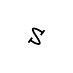
\begin{tikzpicture}[x={(.55ex,0)},y={(0,.55ex)}]
	\draw[smooth, line width=.6pt] (0.9667,0.545) -- (0.8273,0.6541) -- (0.6696,0.7624) -- (0.5,0.866) -- (0.3254,0.961) -- (0.1528,1.043) -- (-0.01133,1.11) -- (-0.1607,1.156) -- (-0.2899,1.181) -- (-0.3945,1.181) -- (-0.471,1.155) -- (-0.5173,1.103) -- (-0.5326,1.025) -- (-0.5173,0.9226) -- (-0.4734,0.7971) -- (-0.4038,0.6515) -- (-0.3127,0.4894) -- (-0.2051,0.3147) -- (-0.08684,0.1318) -- (0.03595,-0.05447) -- (0.1569,-0.2394) -- (0.2696,-0.418) -- (0.3682,-0.5859) -- (0.4473,-0.7388) -- (0.5024,-0.873) -- (0.5299,-0.9855) -- (0.5274,-1.074) -- (0.494,-1.137) -- (0.4299,-1.173) -- (0.3366,-1.184) -- (0.2172,-1.169) -- (0.07558,-1.132) -- (-0.08312,-1.073) -- (-0.253,-0.9971) -- (-0.4276,-0.9068) -- (-0.6001,-0.8063) -- (-0.7635,-0.6994) -- (-0.9113,-0.5902);
	\draw[ line width=.6pt] (-1.18431, -0.959643)--(-0.638322, -0.220787)
								(0.693671, 0.175596)--(1.23965, 0.914452);
\end{tikzpicture}
}

\definition{def:parametrized_surface}{Parametrized Surface}
{Let $\vec r(u,v) = \langle\, f(u,v),g(u,v),h(u,v)\rangle$ be a vector--valued function
that is continuous and one to one on the interior of its domain $R$ in the $u$-$v$ plane. The set of all terminal points of $\vec r$ (i.e., the \emph{range} of $\vec r$\,) is the \sword{surface} \surfaceS, and $\vec r$ along with its domain $R$ form a \sword{parametrization} of \surfaceS.\\

This parametrization is \sword{smooth} on $R$ if $\vec r_u$ and $\vec r_v$ are continuous and $\vec r_u\times \vec r_v$ is never $\vec 0$ on the interior of $R$.\index{surface}\index{parametric equations!of a surface}\index{parametrized surface}\index{smooth!surface}\index{surface!smooth}
}

\mnote{.6}{\textbf{Note:} A function is \emph{one to one} on its domain if the function never repeats an output value over the domain. In the case of $\vec r(u,v)$, $\vec r$ is one to one if $\vec r(u_1,v_1) \neq \vec r(u_2,v_2)$ for all points $(u_1,v_1) \neq (u_2,v_2)$ in the domain of $\vec r$.\index{one to one}
}

Given a point $(u_0,v_0)$ in the domain of a vector--valued function $\vec r$, the vectors $\vec r_u(u_0,v_0)$ and $\vec r_v(u_0,v_0)$ are tangent to the surface \surfaceS\ at $\vec r(u_0,v_0)$ (a proof of this is developed later in this section). The definition of smoothness dictates that $\vec r_u\times \vec r_v \neq \vec 0$; this ensures that neither $\vec r_u$ nor $\vec r_v$ are $\vec 0$, nor are they ever parallel. Therefore smoothness guarantees that $\vec r_u$ and $\vec r_v$ determine a plane that is tangent to \surfaceS.

A surface \surfaceS\ is said to be \sword{orientable}\index{orientable} if a field of normal vectors can be defined on \surfaceS\ that vary continuously along \surfaceS. This definition may be hard to understand; it may help to know that orientable surfaces are often called ``two sided.'' A sphere is an orientable surface, and one can easily envision an ``inside'' and ``outside'' of the sphere. A paraboloid is orientable, where again one can generally envision  ``inside'' and ``outside'' sides (or ``top'' and ``bottom'' sides) to this surface. Just about every surface that one can imagine is orientable, and we'll assume all surfaces we deal with in this text are orientable.

It is enlightening to examine a classic non-orientable surface: the M\"obius band\index{M\"obius band}, shown in Figure \ref{fig:mobius}. Vectors normal to the surface are given, starting at the point indicated in the figure. These normal vectors ``vary continuously'' as they move along the surface. Letting each vector indicate the ``top'' side of the band, we can easily see near any vector which side is the ``top''.

However, if as we progress along the band, we recognize that we are labeling ``both sides'' of the band as the top; in fact, there are not two ``sides'' to this band, but one. The M\"obius band is a non-orientable surface.

\mfigurethree{width=150pt,3Dmenu,activate=onclick,deactivate=onclick,
3Droll=0,
3Dortho=0.009369944222271442,
3Dc2c=0.8152862191200256 -0.5019875168800354 0.28864675760269165,
3Dcoo=11.086544036865234 -8.5783109664917 -7.167413711547852,
3Droo=399.99997970940404,
3Dlights=Headlamp,add3Djscript=asylabels.js}{width=150pt}{.81}{A M\"obius band, a non-orientable surface.}{fig:mobius}{figures/mobius_strip} 

We now practice  parameterizing surfaces. \\

\example{ex_parsurf1}{Parameterizing a surface over a rectangle}
{Parametrize the surface $z=x^2+2y^2$ over the rectangular region $R$ defined by $-3\leq x\leq 3$, $-1\leq y\leq 1$. 
}
{
There is a straightforward way to parametrize a surface of the form $z=f(x,y)$ over a rectangular domain. %Parameterizing surfaces, given in the form $z=f(x,y)$ over rectangular regions is straightforward. 
We  let $x=u$ and $y=v$, and let $\vec r(u,v) = \langle u,v, f(u,v)\rangle$. In this instance, we have $\vec r(u,v) = \langle u,v,u^2+2v^2\rangle$, for $-3\leq u\leq 3$, $-1\leq v\leq 1$. This surface is graphed in Figure \ref{fig:parsurf1}.
\mfigurethree{width=145pt,3Dmenu,activate=onclick,deactivate=onclick,
3Droll=0,
3Dortho=0.005000247620046139,
3Dc2c=0.6257953643798828 0.642341136932373 0.44246822595596313,
3Dcoo=-11.887701988220215 -11.637335777282715 52.40430450439453,
3Droo=399.9999800778292,
3Dlights=Headlamp,add3Djscript=asylabels.js}{width=145pt}{.57}{The surface parametrized in Example \ref{ex_parsurf1}.}{fig:parsurf1}{figures/figparsurf1} 

}\\

\example{ex_parsurf2}{Parameterizing a surface over a circular disk}
{Parametrize the surface $z=x^2+2y^2$ over the circular region $R$ enclosed by the circle of radius 2 that is centered at the origin.
}
{We can parametrize the circular boundary of $R$ with the vector--valued function $\la 2\cos u,2\sin u\ra$, where $0\leq u\leq 2\pi$. We can obtain the interior of $R$ by scaling this function by a variable amount, i.e., by multiplying by $v$: $\la 2v\cos u,2v\sin u\ra$, where $0\leq v\leq 1$. 

It is important to understand the role of $v$ in the above function. When $v=1$, we get the boundary of $R$, a circle of radius 2. When $v=0$, we simply get the point $(0,0)$, the center of $R$ (which can be thought of as a circle with radius of 0). When $v=1/2$, we get the circle of radius $1$ that is centered at the origin, which is the circle \emph{halfway} between the boundary and the center. As $v$ varies from 0 to 1, we create a series of concentric circles that fill out all of $R$.

\mfigurethree{width=145pt,3Dmenu,activate=onclick,deactivate=onclick,
3Droll=0,
3Dortho=0.005000247620046139,
3Dc2c=0.6257953643798828 0.642341136932373 0.44246822595596313,
3Dcoo=-11.887701988220215 -11.637335777282715 52.40430450439453,
3Droo=399.9999800778292,
3Dlights=Headlamp,add3Djscript=asylabels.js}{width=145pt}{.3}{The surface parametrized in Example \ref{ex_parsurf2}.}{fig:parsurf2}{figures/figparsurf2} 

Thus far, we have determined the $x$ and $y$ components of our parametrization of the surface: $x=2v\cos u$ and $y=2v\sin u$. We find the $z$ component simply by using $z = f(x,y) = x^2+2y^2$: 
$$z = (2v\cos u)^2+2(2v\sin u)^2 = 4v^2\cos^2u+8v^2\sin^2u.$$
Thus $\vec r(u,v) = \langle 2v\cos u,2v\sin u,4v^2\cos^2u+8v^2\sin^2u\rangle$, $0\leq u\leq 2\pi$, $0\leq v\leq 1$, which is graphed in Figure \ref{fig:parsurf2}. The way that this graphic was generated highlights how the surface was parametrized. When viewing from above, one can see lines emanating from the origin; they represent different values of $u$ as $u$ sweeps from an angle of 0 up to $2\pi$. One can also see concentric circles, each corresponding to a different value of $v$. 
}\\

Examples \ref{ex_parsurf1} and \ref{ex_parsurf2} demonstrate an important principle when parameterizing surfaces given in the form $z=f(x,y)$ over a region $R$: if one can determine $x$ and $y$ in terms of $u$ and $v$, then $z$ follows directly as $z=f(x,y)$. 

In the following two examples, we parametrize the same surface over triangular regions. Each will use $v$ as a ``scaling factor'' as done in Example \ref{ex_parsurf2}.\\

\example{ex_parsurf3}{Parameterizing a surface over a triangle}
{Parametrize the surface $z=x^2+2y^2$ over the triangular region $R$ enclosed by the coordinate axes and the line $y=2-2x/3$, as shown in Figure \ref{fig:parsurf3}(a). 
}
{We may begin by letting $x=u$, $0\leq u\leq 3$,  and $y = 2-2u/3$. This gives only the line on the ``upper'' side of the triangle. To get all of the region $R$, we can once again scale $y$ by a variable factor, $v$.

Still letting $x = u$, $0\leq u\leq 3$, we let $y = v(2-2u/3)$, $0\leq v\leq 1$. When $v=0$, all $y$-values are 0, and we get the portion of the $x$-axis between $x=0$ and $x=3$. When $v=1$, we get the upper side of the triangle. When $v=1/2$, we get the line $y=1/2(2-2u/3) = 1-u/3$, which is the line ``halfway up'' the triangle, shown in the figure with a dashed line.

\mtable{.65}{Part (a) shows a graph of the region $R$, and part (b) shows the surface over $R$, as defined in Example \ref{ex_parsurf3}.}{fig:parsurf3}
{\begin{tabular}{c}
\myincludegraphics{figures/figparsurf3a}\\[-5pt]
(a)\\[10pt]
\myincludegraphicsthree{width=145pt,3Dmenu,activate=onclick,deactivate=onclick,
3Droll=0,
3Dortho=0.005000247620046139,
3Dc2c=0.6257953643798828 0.642341136932373 0.44246822595596313,
3Dcoo=-11.887701988220215 -11.637335777282715 52.40430450439453,
3Droo=399.9999800778292,
3Dlights=Headlamp,add3Djscript=asylabels.js}{width=145pt}{figures/figparsurf3}\\
(b)
\end{tabular}
}

Letting $z = f(x,y) = x^2+2y^2$, we have $\vec r(u,v) = \langle u, v(2-2u/3), u^2+2\big(v(2-2u/3)\big)^2\rangle$, $0\leq u\leq 3$, $0\leq v\leq 1$. This surface is graphed in Figure \ref{fig:parsurf3}(b). Again, when one looks from above, we can see the scaling effects of $v$: the series of lines that run to the point $(3,0)$ each represent a different value of $v$.

Another common way to parametrize the surface is to begin with $y=u$, $0\leq u\leq 2$. Solving the equation of the line $y=2-2x/3$ for $x$, we have $x = 3-3y/2$, leading to using $x=v(3-3u/2)$, $0\leq v\leq 1$. With $z=x^2+2y^2$, we have $\vec r(u,v) = \langle v(3-3u/2),u, \big(v(3-3u/2)\big)^2+2v^2\rangle$, $0\leq u\leq 2$, $0\leq v\leq 1$.
}\\

\example{ex_parsurf4}{Parameterizing a surface over a triangle}
{Parametrize the surface $z=x^2+2y^2$ over the triangular region $R$ enclosed by the  lines $y=3-2x/3$, $y=1$ and $x=0$ as shown in Figure \ref{fig:parsurf4}(a). 
}
{While the region $R$ in this example is very similar to the region $R$ in the previous example, and our method of parameterizing the surface is fundamentally the same, it will feel as though our answer is much different than before.

We begin with letting $x=u$, $0\leq u\leq 3$. We may be tempted to let $y = v(3-2u/3)$, $0\leq v\leq 1$, but this is incorrect. When $v = 1$, we obtain the upper line of the triangle as desired. However, when $v=0$, the $y$-value is 0, which does not lie in the region $R$. 


We will describe the general method of proceeding following this example. For now, consider $y = 1+v(2-2u/3)$, $0\leq v\leq 1$. Note that when $v=1$, we have $y=3-2u/3$, the upper line of the boundary of $R$. Also, when $v=0$, we have $y=1$, which is the lower boundary of $R$. With $z=x^2+2y^2$, we determine $\vec r(u,v) = \langle u, 1+v(2-2u/3), u^2+2\big(1+v(2-2u/3)\big)^2\rangle$, $0\leq u\leq 3$, $0\leq v\leq 1$. 

The surface is graphed in Figure \ref{fig:parsurf4}(b).
\mtable{.68}{Part (a) shows a graph of the region $R$, and part (b) shows the surface over $R$, as defined in Example \ref{ex_parsurf4}.}{fig:parsurf4}
{\begin{tabular}{c}
\myincludegraphics{figures/figparsurf4a}\\[-5pt]
(a)\\[10pt]
\myincludegraphicsthree{width=145pt,3Dmenu,activate=onclick,deactivate=onclick,
3Droll=0,
3Dortho=0.005000247620046139,
3Dc2c=0.6257953643798828 0.642341136932373 0.44246822595596313,
3Dcoo=-11.887701988220215 -11.637335777282715 52.40430450439453,
3Droo=399.9999800778292,
3Dlights=Headlamp,add3Djscript=asylabels.js}{width=145pt}{figures/figparsurf4}\\
(b)
\end{tabular}
}
}\\

Given a surface of the form $z=f(x,y)$, one can often determine a parametrization of the surface over a region $R$ in a manner similar to determining bounds of integration over a region $R$. Using the techniques of Section \ref{sec:iterated_integrals}, suppose a region $R$ can be described by $a\leq x\leq b$, $g_1(x) \leq y\leq g_2(x)$, i.e., the area of $R$ can be found using the iterated integral
$$\int_a^b\int_{g_1(x)}^{g_2(x)}\ dy\ dx.$$

When parameterizing the surface, we can let $x=u$, $a\leq u\leq b$, and we can let $y = g_1(u)+v\big(g_2(u)-g_1(u)\big)$, $0\leq v\leq 1$. The parametrization of $x$ is straightforward, but look closely at how $y$ is determined. When $v=0$, $y=g_1(u) = g_1(x)$. When $v=1$, $y= g_2(u)=g_2(x)$. 


 As a specific example, consider the triangular region $R$ from Example \ref{ex_parsurf4}, shown in Figure \ref{fig:parsurf4}(a). Using the techniques of Section \ref{sec:iterated_integrals}, we can find the area of $R$ as
$$\int_0^3\int_1^{3-2x/3} dy\ dx.$$
Following the above discussion, we can set $x=u$, where $0\leq u\leq 3$, and set $y = 1+ v\big(3-2u/3-1\big) = 1+v(2-2u/3)$, $0\leq v\leq 1$, as used in that example.

One can do a similar thing if $R$ is bounded by $c\leq y\leq d$, $h_1(y)\leq x\leq h_2(y)$, but for the sake of simplicity we leave it to the reader to flesh out those details. The principles outlined above are given in the following Key Idea for reference.

\keyidea{idea:parameterizing_surfaces}{Parameterizing Surfaces}
{Let a surface \surfaceS\ be the graph of a function $z=f(x,y)$, where the domain of $f$ is  a closed, bounded region $R$ in the $x$-$y$ plane. 
%be the portion of the graph of $z=f(x,y)$ that lies above a region $R$ in the $x$-$y$ plane. 
Let $R$ be bounded by $a\leq x\leq b$, $g_1(x)\leq y\leq g_2(x)$, i.e., the area of $R$ can be found using the iterated integral $\int_a^b\int_{g_1(x)}^{g_2(x)}\ dy\ dx$, and let $h(u,v) = g_1(u)+v\big(g_2(u)-g_1(u)\big)$. 

\surfaceS\ can be parametrized as 
$$\vec r(u,v) = \la u, h(u,v), f\big(u,h(u,v)\big)\ra,\quad a\leq u\leq b,\ 0\leq v\leq 1.$$
}\\

\example{ex_parsurf5}{Parameterizing a cylinderical surface}
{Find a parametrization of the cylinder $x^2 + z^2/4=1$, where $-1\leq y\leq 2$, as shown in Figure \ref{fig:parsurf5}. 
}
{The equation $x^2+z^2/4=1$ can be envisioned to describe an ellipse in the $x$-$z$ plane; as the equation lacks a $y$-term, the equation describes a cylinder (recall Definition \ref{def:cylinder}) that extends without bound parallel to the $y$-axis. This ellipse has a vertical major axis of length 4, a horizontal minor axis of length 2, and is centered at the origin. We can parametrize this ellipse using sines and cosines; our parametrization can begin with
$$\vec r(u,v) = \la \cos u, \text{???}, 2\sin u\ra,\quad 0\leq u\leq 2\pi,$$
where we still need to determine the $y$ component.

\mfigurethree{width=150pt,3Dmenu,activate=onclick,deactivate=onclick,
3Droll=0,
3Dortho=0.004427968058735132,
3Dc2c=0.8313615918159485 0.5262497067451477 0.17860320210456848,
3Dcoo=1.6293458938598633 13.199743270874023 -3.546671152114868,
3Droo=399.9999708739728,
3Dlights=Headlamp,add3Djscript=asylabels.js}{width=150pt}{.65}{The cylinder parametrized in Example \ref{ex_parsurf5}.}{fig:parsurf5}{figures/figparsurf5} 

While the cylinder $x^2+z^2/4=1$ is satisfied by any $y$ value, the problem states that all $y$ values are to be between $y=-1$ and $y=2$. Since the value of $y$ does not depend at all on the values of $x$ or $z$, we can use another variable, $v$, to describe $y$. Our final answer is
$$\vec r(u,v) = \la \cos u, v, 2\sin u\ra, \quad 0\leq u\leq 2\pi,\quad -1\leq v\leq 2.$$
\vskip-1.5\baselineskip
}\\

\example{ex_parsurf6}{Parameterizing an elliptic cone}
{Find a parametrization of the elliptic cone $z^2 = \frac{x^2}{4}+\frac{y^2}{9}$, where $-2\leq z\leq 3$, as shown in Figure \ref{fig:parsurf6a}.
}
{One way to parametrize this cone is to recognize that given a $z$ value, the cross section of the cone at that $z$ value is an ellipse with equation $\frac{x^2}{(2z)^2} + \frac{y^2}{(3z)^2}=1$. We can let $z=v$, for $-2\leq v\leq 3$ and then parametrize the above ellipses using sines, cosines and $v$.
\mfigurethree{width=150pt,3Dmenu,activate=onclick,deactivate=onclick,
3Droll=0,
3Dortho=0.00452691363170743,
3Dc2c=0.625795304775238 0.642341136932373 0.44246816635131836,
3Dcoo=0.0026521924883127213 4.370458126068115 12.347787857055664,
3Droo=399.9999637774216,
3Dlights=Headlamp,add3Djscript=asylabels.js}{width=150pt}{.35}{The elliptic cone as described in  Example \ref{ex_parsurf6}.}{fig:parsurf6a}{figures/figparsurf6a}

We can parametrize the $x$ component of our surface with $x=2z\cos u$ and the $y$ component with $y=3z\sin u$, where $0\leq u\leq 2\pi$. Putting all components together, we have
$$\vec r(u,v) = \la 2v\cos u, 3v\sin u, v\ra,\quad 0\leq u\leq 2\pi,\quad -2\leq v\leq 3.$$

%\mtable{.68}{An elliptic cone in (a), drawn again in (b) with its domain restricted, as described in  Example \ref{ex_parsurf6}.}{fig:parsurf6}
%{\begin{tabular}{c}
%\myincludegraphicsthree{width=145pt,3Dmenu,activate=onclick,deactivate=onclick,
%3Droll=0,
%3Dortho=0.00452691363170743,
%3Dc2c=0.625795304775238 0.642341136932373 0.44246816635131836,
%3Dcoo=0.0026521924883127213 4.370458126068115 12.347787857055664,
%3Droo=399.9999637774216,
%3Dlights=Headlamp,add3Djscript=asylabels.js}{scale=1}{figures/figparsurf6a}\\
%(a)\\[10pt]
%\myincludegraphicsthree{width=145pt,3Dmenu,activate=onclick,deactivate=onclick,
%3Droll=0,
%3Dortho=0.00452691363170743,
%3Dc2c=0.625795304775238 0.642341136932373 0.44246816635131836,
%3Dcoo=0.0026521924883127213 4.370458126068115 12.347787857055664,
%3Droo=399.9999637774216,
%3Dlights=Headlamp,add3Djscript=asylabels.js}{scale=1}{figures/figparsurf6b}\\
%(b)
%\end{tabular}
%}


When $v$ takes on negative values, the radii of the cross--sectional ellipses become ``negative,'' which can lead to some surprising results. Consider Figure \ref{fig:parsurf6b}, where the cone is graphed for $0\leq u\leq \pi$. Because $v$ is negative below the $x$-$y$ plane, the radii of the cross--sectional ellipses are negative, and the opposite side of the cone is sketched below the $x$-$y$ plane.
\mfigurethree{width=150pt,3Dmenu,activate=onclick,deactivate=onclick,
3Droll=0,
3Dortho=0.00452691363170743,
3Dc2c=0.625795304775238 0.642341136932373 0.44246816635131836,
3Dcoo=0.0026521924883127213 4.370458126068115 12.347787857055664,
3Droo=399.9999637774216,
3Dlights=Headlamp,add3Djscript=asylabels.js}{width=150pt}{.78}{The elliptic cone as described in  Example \ref{ex_parsurf6} with restricted domain.}{fig:parsurf6b}{figures/figparsurf6b}
}\\

\example{ex_parsurf7}{Parameterizing an ellipsoid}
{Find a parametrization of the ellipsoid $\frac{x^2}{25}+y^2+\frac{z^2}{4}=1$ as shown in Figure \ref{fig:parsurf7}(a).
}
{Recall Key Idea \ref{idea:unit_vectors} from Section \ref{sec:vector_intro}, which states that all unit vectors in space have the form $\langle \sin\theta\cos\varphi,\sin\theta\sin\varphi,\cos\theta\rangle$ for some angles $\theta$ and $\varphi$. If we choose our angles appropriately, this allows us to draw the unit sphere. To get an ellipsoid, we need only scale each component of the sphere appropriately.

The $x$-radius of the given ellipsoid is 5, the $y$-radius is 1 and the $z$-radius is 2. Substituting $u$ for $\theta$ and $v$ for $\varphi$, we have $\vec r(u,v) = \langle 5\sin u\cos v, \sin u\sin v,2\cos u\rangle$, where we still need to determine the ranges of $u$ and $v$. 

Note how the $x$ and $y$ components of $\vec r$ have  $\cos v$ and $\sin v$ terms, respectively. This hints at the fact that ellipses are drawn parallel to the $x$-$y$ plane as $v$ varies, which implies we should have $v$ range from $0$ to $2\pi$. 

One may be tempted to let $0\leq u\leq 2\pi$ as well, but note how the $z$ component is $2\cos u$. We only need $\cos u$ to take on values between $-1$ and $1$ once, therefore we can restrict $u$ to $0\leq u\leq \pi$. 

\mtable{.4}{An ellipsoid in (a), drawn again in (b) with its domain restricted, as described in  Example \ref{ex_parsurf7}.}{fig:parsurf7}
{\begin{tabular}{c}
\myincludegraphicsthree{width=145pt,3Dmenu,activate=onclick,deactivate=onclick,
3Droll=0,
3Dortho=0.00452691363170743,
3Dc2c=0.625795304775238 0.642341136932373 0.44246816635131836,
3Dcoo=0.0026521924883127213 4.370458126068115 12.347787857055664,
3Droo=399.9999637774216,
3Dlights=Headlamp,add3Djscript=asylabels.js}{width=145pt}{figures/figparsurf7a}\\
(a)\\[10pt]
\myincludegraphicsthree{width=145pt,3Dmenu,activate=onclick,deactivate=onclick,
3Droll=0,
3Dortho=0.00452691363170743,
3Dc2c=0.625795304775238 0.642341136932373 0.44246816635131836,
3Dcoo=0.0026521924883127213 4.370458126068115 12.347787857055664,
3Droo=399.9999637774216,
3Dlights=Headlamp,add3Djscript=asylabels.js}{width=145pt}{figures/figparsurf7b}\\
(b)
\end{tabular}
}

The final parametrization is thus
$$\vec r(u,v) = \langle 5\sin u\cos v, \sin u\sin v,2\cos u\rangle, \quad 0\leq u\leq\pi,\quad 0\leq v\leq 2\pi.$$

In Figure \ref{fig:parsurf7}(b), the ellipsoid is graphed on $\frac{\pi}{4}\leq u\leq \frac{2\pi}{3}$, $\frac{\pi}4\leq v\leq \frac{3\pi}2$ to demonstrate how each variable affects the surface.
}\\

Parametrization is a powerful way to represent surfaces. One of the advantages of the methods of parametrization described in this section is that the domain of $\vec r(u,v)$ is always a rectangle; that is, the bounds on $u$ and $v$ are constants. This will make some of our future computations easier to evaluate.

Just as we could parametrize curves in more than one way, there will always be multiple ways to parametrize a surface. Some ways will be more ``natural'' than others, but these other ways are not incorrect. Because technology is often readily available, it is often a good idea to check one's work by graphing a parametrization of a surface to check if it indeed represents what it was intended to.

\vskip \baselineskip
\noindent\textbf{\large Surface Area}\\

It will become important in the following sections to be able to compute the surface area of a surface \surfaceS\ given a smooth parametrization $\vec r(u,v)$, $a\leq u\leq b$, $c\leq v\leq d$. Following the principles given in the integration review at the beginning of this chapter, we can say that\index{surface area!of parametrized surface}
$$\text{Surface Area of \surfaceS}=S = \iint_{\surfaceS}\ dS,$$
where $dS$ represents a small amount of surface area. That is, to compute total surface area $S$, add up lots of small amounts of surface area $dS$ across the entire surface \surfaceS. The key to finding surface area is knowing how to compute $dS$. We begin by approximating.

In Section \ref{sec:surface_area} we used the area of a plane to approximate the surface area of a small portion of a surface. We will do the same here.

Let $R$ be the region of the $u$-$v$ plane bounded by $a\leq u\leq b$, $c\leq v\leq d$ as shown in Figure \ref{fig:parsurfarea}(a). Partition $R$ into rectangles of width $\Delta u = \frac{b-a}n$ and height $\Delta v = \frac{d-c}n$, for some $n$. Let $p=(u_0,v_0)$ be the lower left corner of some rectangle in the partition, and let $m$ and $q$ be neighboring corners as shown.

The point $p$ maps to a point $P = \vec r(u_0,v_0)$ on the surface \surfaceS, and the rectangle with corners $p$, $m$ and $q$ maps to some region (probably not rectangular) on the surface as shown in Figure \ref{fig:parsurfarea}(b), where $M = \vec r(m)$ and $Q = \vec r(q)$. We wish to approximate the surface area of this mapped region.

Let $\vec u = M-P$ and $\vec v = Q-P$. These two vectors form a parallelogram, illustrated in Figure \ref{fig:parsurfarea}(c), whose area \emph{approximates} the surface area we seek. In this particular illustration, we can see that parallelogram does not particularly match well the region we wish to approximate, but that is acceptable; by increasing the number of partitions of $R$, $\Delta u$ and $\Delta v$ shrink and our approximations will become better.

\mtable{.57}{Illustrating the process of finding surface area by approximating with planes.}{fig:parsurfarea}
{\begin{tabular}{c}
\myincludegraphics{figures/figparsurfareaC}\\[-5pt]
(a)\\[10pt]
\myincludegraphicsthree{width=145pt,3Dmenu,activate=onclick,deactivate=onclick,
3Droll=0,
3Dortho=0.004750744439661503,
3Dc2c=0.6291605234146118 0.6371588706970215 0.4451805353164673,
3Dcoo=84.20735168457031 80.18836212158203 107.64490509033203,
3Droo=133.06991885752157,
3Dlights=Headlamp,add3Djscript=asylabels.js}{width=145pt}{figures/figparsurfareaA}\\
(b)\\[10pt]
\myincludegraphicsthree{width=145pt,3Dmenu,activate=onclick,deactivate=onclick,
3Droll=0,
3Dortho=0.003687552874907851,
3Dc2c=0.5666888952255249 0.6642887592315674 0.48742610216140747,
3Dcoo=145.19125366210938 160.48304748535156 209.22018432617188,
3Droo=135.59128411404498,
3Dlights=Headlamp,add3Djscript=asylabels.js}{width=145pt}{figures/figparsurfareaB}\\
(c)
\end{tabular}
}

From Section \ref{sec:cross_product} we know the area of this parallelogram is $\snorm{\vec u\times \vec v}$. If we repeat this approximation process for each rectangle in the partition of $R$, we can sum the areas of all the parallelograms to get an approximation of the surface area $S$:
$$\text{Surface area of \surfaceS} =S \approx \sum_{j=1}^n\sum_{i=1}^n \snorm{\vec u_{i,j}\times \vec v_{i,j}},$$
where $\vec u_{i,j} = \vec r(u_i+\Delta u,v_j) - \vec r(u_i,v_j)$ and $\vec v_{i,j} = \vec r(u_i,v_j+\Delta v)-\vec r(u_i,v_j)$.

From our previous calculus experience, we expect that taking a limit as $n\to \infty$ will result in the exact surface area. However, the current form of the above double sum makes it difficult to realize what the result of that limit is. The following rewriting of the double summation will be helpful:

\begin{align*}
&\sum_{j=1}^n\sum_{i=1}^n \snorm{\vec u_{i,j}\times \vec v_{i,j}}= \\ 
&\sum_{j=1}^n\sum_{i=1}^n \snorm{\big(\vec r(u_i+\Delta u,v_j) - \vec r(u_i,v_j)\big) \times \big(\vec r(u_i,v_j+\Delta v)-\vec r(u_i,v_j)\big)}= \\
&\sum_{j=1}^n\sum_{i=1}^n \snorm{\frac{\vec r(u_i+\Delta u,v_j) - \vec r(u_i,v_j)}{\Delta u} \times \frac{\vec r(u_i,v_j+\Delta v)-\vec r(u_i,v_j)}{\Delta v}}\Delta u\Delta v.
\end{align*}

We now take the limit as $n\to\infty$, forcing $\Delta u$ and $\Delta v$ to 0. As $\Delta u\to 0$,
$$\frac{\vec r(u_i+\Delta u,v_j) - \vec r(u_i,v_j)}{\Delta u}\quad \to\quad \vec r_u(u_i,v_j)\quad \text{ and} $$
$$\frac{\vec r(u_i,v_j+\Delta v)-\vec r(u_i,v_j)}{\Delta v}\quad \to\quad \vec r_v(u_i,v_j).$$
(This limit process also demonstrates that $\vec r_u(u,v)$ and $\vec r_v(u,v)$ are tangent to the surface \surfaceS\ at $\vec r(u,v)$. We don't need this fact now, but it will be important in the next section.)

Thus, in the limit, the double sum leads to a double integral:
$$\lim_{n\to\infty} \sum_{j=1}^n\sum_{i=1}^n \snorm{\vec u_{i,j}\times \vec v_{i,j}}= \int_c^d\int_a^b \snorm{\vec r_u\times\vec r_v}\ du\ dv.$$

\theorem{thm:par_surface_area}{Surface Area of Parametrically Defined Surfaces}
{Let $\vec r(u,v)$ be a smooth parametrization of a surface \surfaceS\ over a closed, bounded region $R$ of the $u$-$v$ plane.\index{surface area!of parametrized surface} 
\begin{itemize}
\item	The surface area differential $dS$ is: $dS = \snorm{\vec r_u\times \vec r_v}\ dA$.
\item The surface area $S$ of \surfaceS\ is
$$S = \iint_\surfaceS\ dS = \iint_R \snorm{\vec r_u\times \vec r_v}\ dA.$$
\end{itemize}
}
%\mnote{.4}{\textbf{Note:} In Definition \ref{def:surfacearea}, the surface area differential of a surface given in the form $z=f(x,y)$ is defined to be $dS = \sqrt{1+f_x^2+f_y^2}\ dA$. We can use this differential in this and subsequent sections, though 

\example{ex_parsurfarea1}{Finding the surface area of a parametrized surface}
{Using the parametrization found in Example \ref{ex_parsurf2}, find the surface area of $z=x^2+2y^2$ over the circular disk of radius 2, centered at the origin.
}
{In Example \ref{ex_parsurf2}, we parametrized the surface as $\vec r(u,v) = \la 2v\cos u, 2v\sin u, 4v^2\cos^2u+8v^2\sin^2u\ra$, for $0\leq u\leq 2\pi$, $0\leq v\leq 1$. To find the surface area using Theorem \ref{thm:par_surface_area}, we need $\snorm{\vec r_u\times\vec r_v}$. We find:
\begin{align*}
\vec r_u &= \la -2v\sin u, 2v\cos u, 8v^2\cos u\sin u\ra\\
\vec r_v &= \la 2\cos u, 2\sin v, 8v\cos^2 u+16v\sin^2u\ra\\
\vec r_u\times\vec r_v &= \la 16v^2\cos u, 32v^2\sin u, -4v\ra\\
\snorm{\vec r_u\times\vec r_v} &= \sqrt{256v^4\cos^2u+1024v^4\sin^2u+16v^2}.
\end{align*}
Thus the surface area is
\begin{align*}
S = \iint_\surfaceS \ dS &= \iint_R\snorm{\vec r_u\times \vec r_v}\ dA \\
& = \int_0^1\int_0^{2\pi} \sqrt{256v^4\cos^2u+1024v^4\sin^2u+16v^2}\ du\ dv \approx 53.59.
\end{align*}
There is a lot of tedious work in the above calculations and the final integral is nontrivial. The use of a computer-algebra system is highly recommended.
}\\

In Section \ref{sec:line_int_intro}, we recalled the arc length differential $ds=\snorm{\vrp(t)}dt$. In subsequent sections, we used that differential, but in most applications the ``$\snorm{\vrp(t)}$'' part of the differential canceled out of the integrand (to our benefit, as integrating the square roots of functions is generally difficult). We will find a similar thing happens when we use the surface area differential $dS$ in the following sections. That is, our main goal is not to be able to compute surface area; rather, surface area is a tool to obtain other quantities that are more important and useful. In our applications, we will use $dS$, but most of the time the ``$\snorm{\vec r_u\times \vec r_v}$'' part will cancel out of the integrand, making the subsequent integration easier to compute.

\printexercises{exercises/14_05_exercises}